\chapter{Design Front-End}

%capo la mia conoscenza di latex si sta espandendo però probabilmente questo non compila comunque, halp me plz
% ho fatto del mio meglio per preparare un brodo degno di gordon ramsay
% by @Boss314

\section{Pagina Iniziale}

    \label{fig:4.1}
    \begin{figure}[H]
        \center
        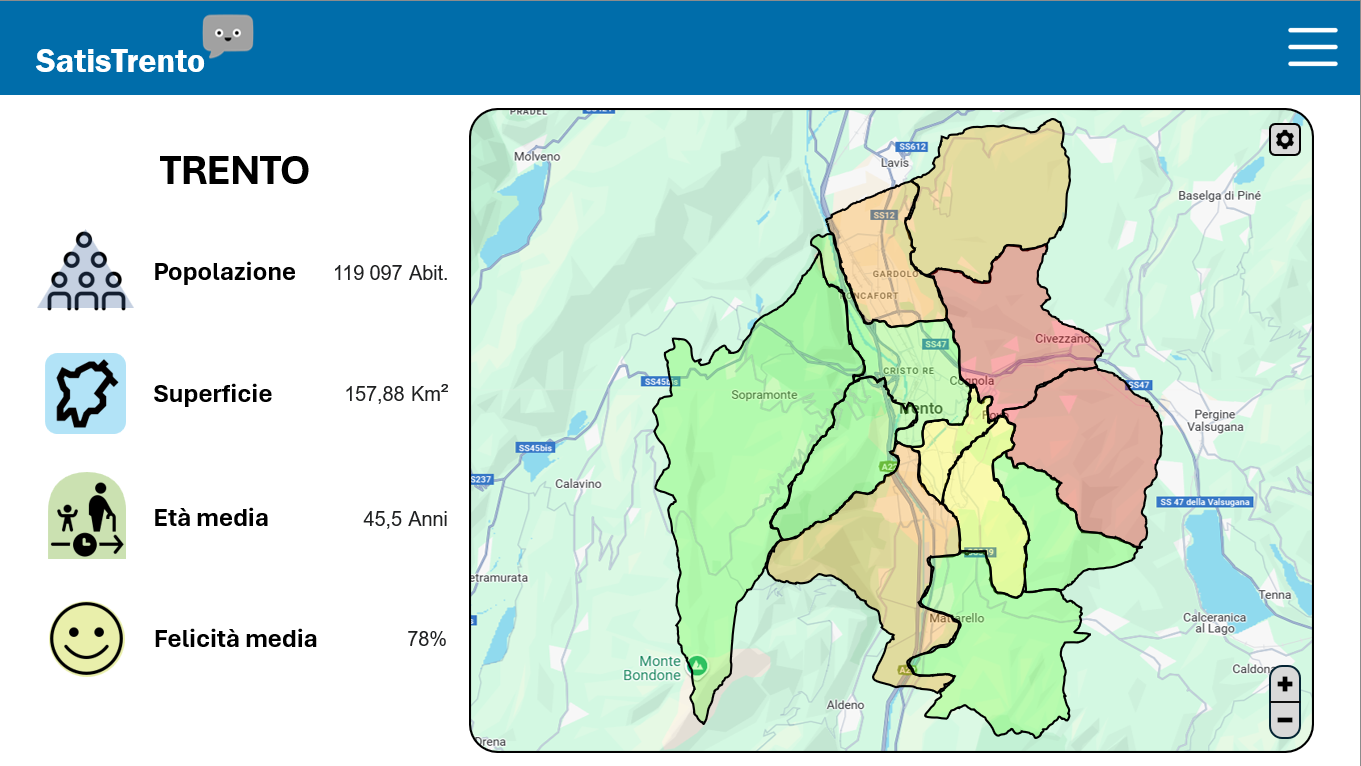
\includegraphics[width=0.6\textwidth]{Interfaccia_grafica/VisCitta.png}
        \caption{Schermata principale dell'applicazione}
    \end{figure}

    La Figura 4.1 mostra un mockup della pagina principale dell'applicazione, questa schermata sarà visibile a tutti gli utenti, loggati e non loggati.

    \begin{itemize}
        \item \textbf{RF1: Visualizzazione città} \begin{itemize}
            \item La homepage dell'applicazione mostra gli attributi della città con a fianco la mappa del Comune di Trento divisa attraverso le circoscrizioni.
        \end{itemize}
        \item \textbf{RF2: Interazione con la mappa} \begin{itemize} 
            \item Ai lati della mappa della città vengono visualizzati i pulsanti per la modifica del focus e quello per la modifica delle impostazioni.
        \end{itemize}
        \item \textbf{RF5: Multi lingua} \begin{itemize} 
            \item Attraverso l'utilizzo del menù a tendina presente nella header è possibile cambiare la lingua preselezionata, ovvero l'italiano.
        \end{itemize}
        \item \textbf{RF6: Login} \begin{itemize} 
            \item Attraverso l'utilizzo del menù a tendina presente nella header è possibile accedere all'account personale. Questo permette agli utenti non loggati di accedere al proprio account tramite servizi Single Sign On.
        \end{itemize}
        \item \textbf{RNF10: Facilità d'uso} \begin{itemize}
                \item La grafica disponibile a tutti gli utenti presenta un design chiaro, usando icone per rendere la navigazione attraverso la web-app il più accessibile e intuitiva possibile.
        \end{itemize}
        \item \textbf{RNF11: Facilità di navigazione} \begin{itemize}
            \item L'interfaccia permette all'utente di navigare facilmente tra le pagine, inoltre è possibile accedere a tutte le funzionalità fornite all'utente selezionato tramite un menù a tendina, che si aprirà cliccando sull'icona ad "hamburger" presente nella parte superiore destra della schermata.
        \end{itemize}
        \item \textbf{RNF12: Multilingua} \begin{itemize} 
            \item All'inizio, l'interfaccia sarà presentata in lingua italiana. Il design include pulsanti, sempre presenti nella parte alta della schermata, per cambiare la lingua in inglese o tedesco.
        \end{itemize}
    \end{itemize}


\newpage
\section{Utente Loggato, Dati in Tabella}

    \begin{figure}[H]
        \center
        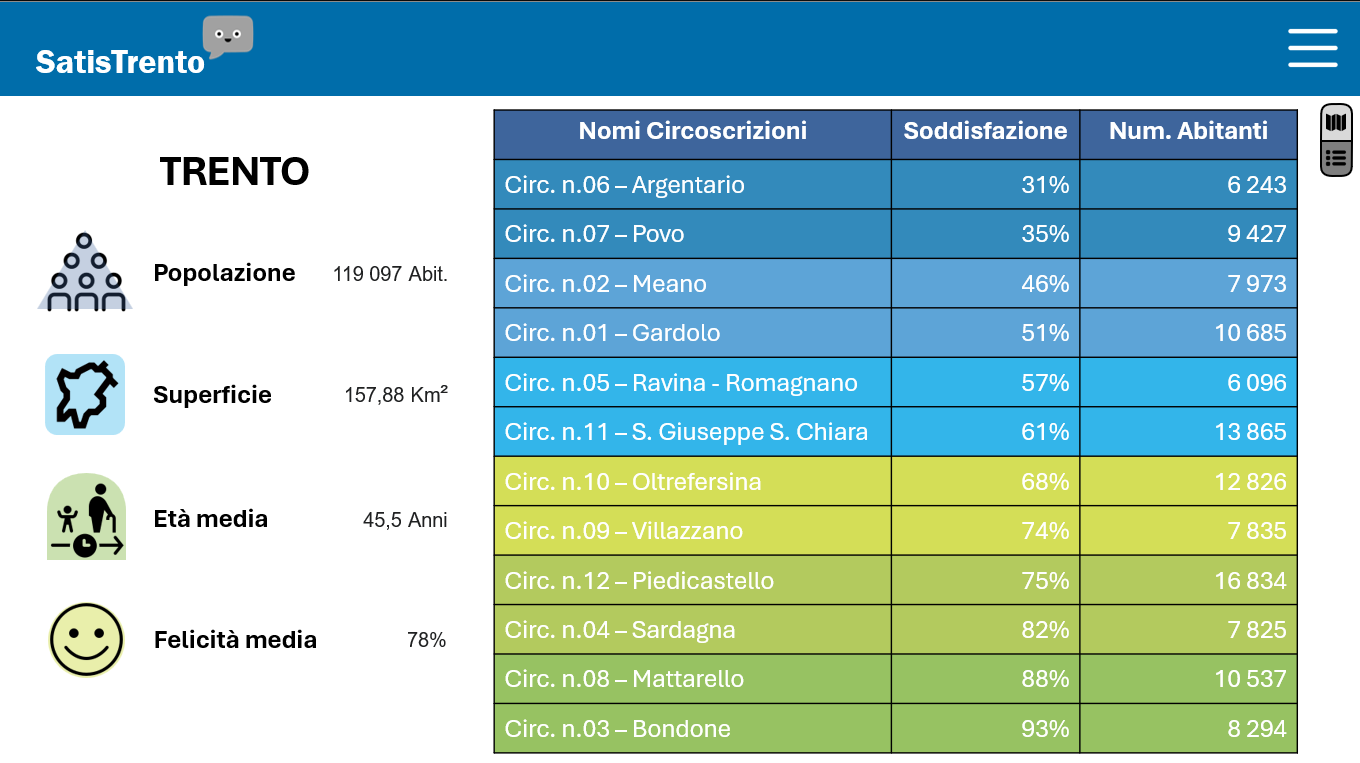
\includegraphics[width=0.6\textwidth]{Interfaccia_grafica/VisCittaLogin.png}
        \caption{Dettaglio dati per analisti e amministratori}
    \end{figure}    

    La Figura 4.2 mostra il mockup della schermata di homepage modificata visibile agli utenti di tipo analista,questa schermata sarà visibile solo dopo che l'utente ha effettuato l'accesso.

    
    \begin{itemize}
        \item \textbf{RF2: Interazione con la mappa} \begin{itemize}
            \item La seguente visualizzazione è possibile soltanto perchè si ha prima interagito con il pulsante per la modifica della mappa.
        \end{itemize}
        \item \textbf{RF7: Logout} \begin{itemize} 
            \item Attraverso l'utilizzo del menù a tendina presente nella header è possibile eseguire il processo di scollegamento dall'account personale.
        \end{itemize}
        \item \textbf{RF12: Interazione con la tabella} \begin{itemize} 
            \item Attraverso la tabella mostrata in figura sarà possibile per gli utenti analisti ordinare le circoscrizioni e i quartieri attraverso un attributo tra quelli presenti a piacimento.
        \end{itemize}
        \item \textbf{RNF10: Facilità d'uso} \begin{itemize}
            \item L'interfaccia è stata progettata per essere il più intuitiva possibile, i dati sono presentati in una tabella la quale potrà essere ordinata e filtrata per facilitare la consultazione. Il tutto tramite pulsanti e icone facilmente riconoscibili. Quali le icone di "mappa" e "tabella" per cambiare la visualizzazione dei dati, oppure le icone di "freccia" per ordinare i dati in base a una colonna specifica.
        \end{itemize}
        \item \textbf{RNF11: Facilità di navigazione} \begin{itemize}
            \item L'interfaccia permette all'utente di navigare facilmente tra le pagine, inoltre è possibile accedere a tutte le funzionalità dell'applicazione tramite il menù a tendina, che si apre cliccando sull'icona standard ad "hamburger" presente nella parte superiore destra della schermata.
            \end{itemize}
    \end{itemize}
\newpage
\section{Selezione di un Quartiere}
    \begin{figure}[H]
        \center
        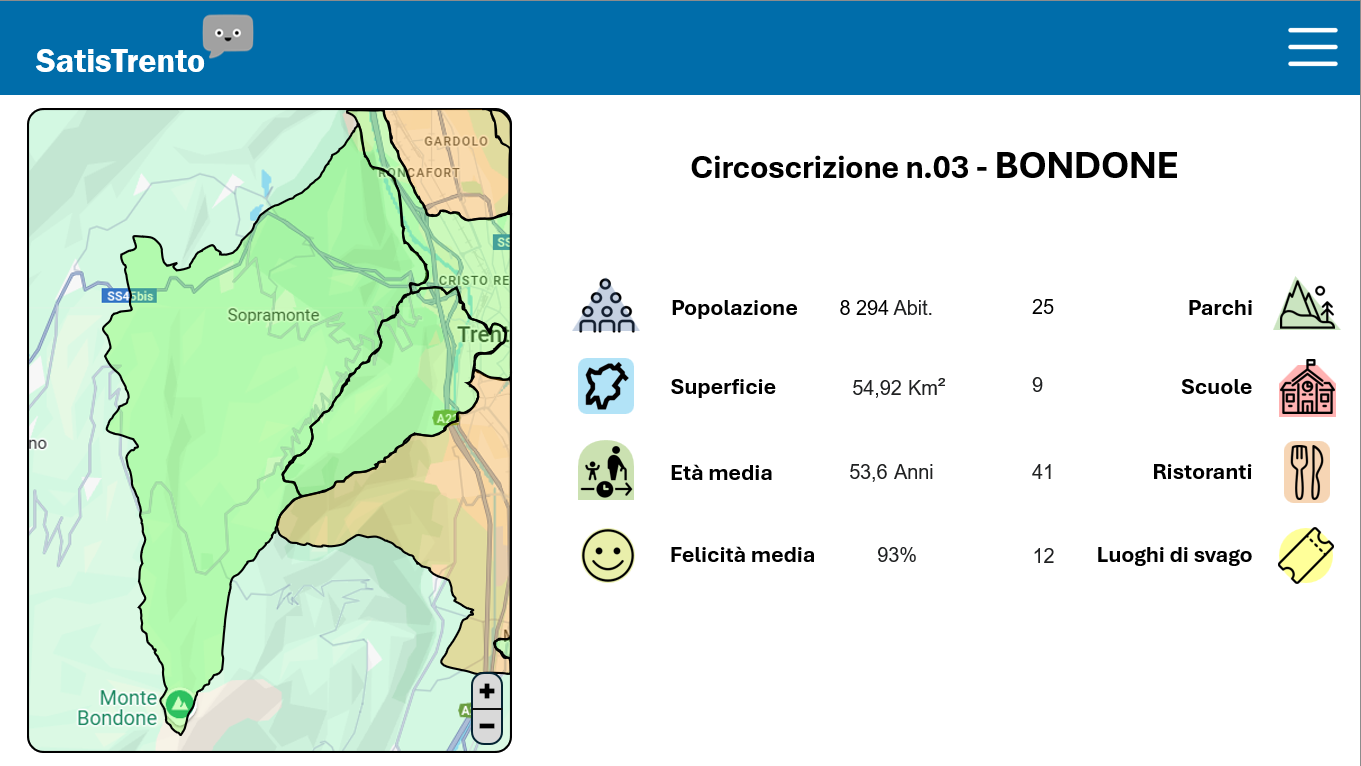
\includegraphics[width=0.6\textwidth]{Interfaccia_grafica/VisCircoscrizione.png}
        \caption{Dettaglio dati per un quartiere selezionato}
    \end{figure}    

    La Figura 4.3 mostra il mockup della schermata visibile dopo che l'utente ha cliccato su una delle circoscrizione presenti nella mappa o nella tabella.

    \begin{itemize}
        \item \textbf{RF3: Visualizzazione zona} \begin{itemize}
            \item La visualizzazione della circoscrizione selezionata presenta gli attributi ed i servizi al cittadino appartenente alla seguente circoscrizione con al fianco la visualizzazione, tramite mappa, del territorio selezionato e del suo circondario.
        \end{itemize}
        \item \textbf{RF4: Elenco strutture} \begin{itemize}
            \item Nel caso in cui si selezionasse uno degli attributi facente parte dei servizi, in questo caso: Parchi, Scuole, Ristoranti, Luoghi di svago, verrebbe mostrato a schermo l'elenco delle strutture che adempiono a fornire tale servizio.
        \end{itemize}
        \item \textbf{RF13: Accesso completo agli attributi} \begin{itemize}
            \item Nel caso in cui si avesse fatto l'accesso come analista nella seguente interfaccia sarebbe stato presente anche un menù per la selezione della categoria degli attributi che si voleva visualizzare.
        \end{itemize}
    \end{itemize}
\section{Caricamento sondaggi e modifica dati}
    \label{fig:4.4}
    \begin{figure}[H]
        \center
        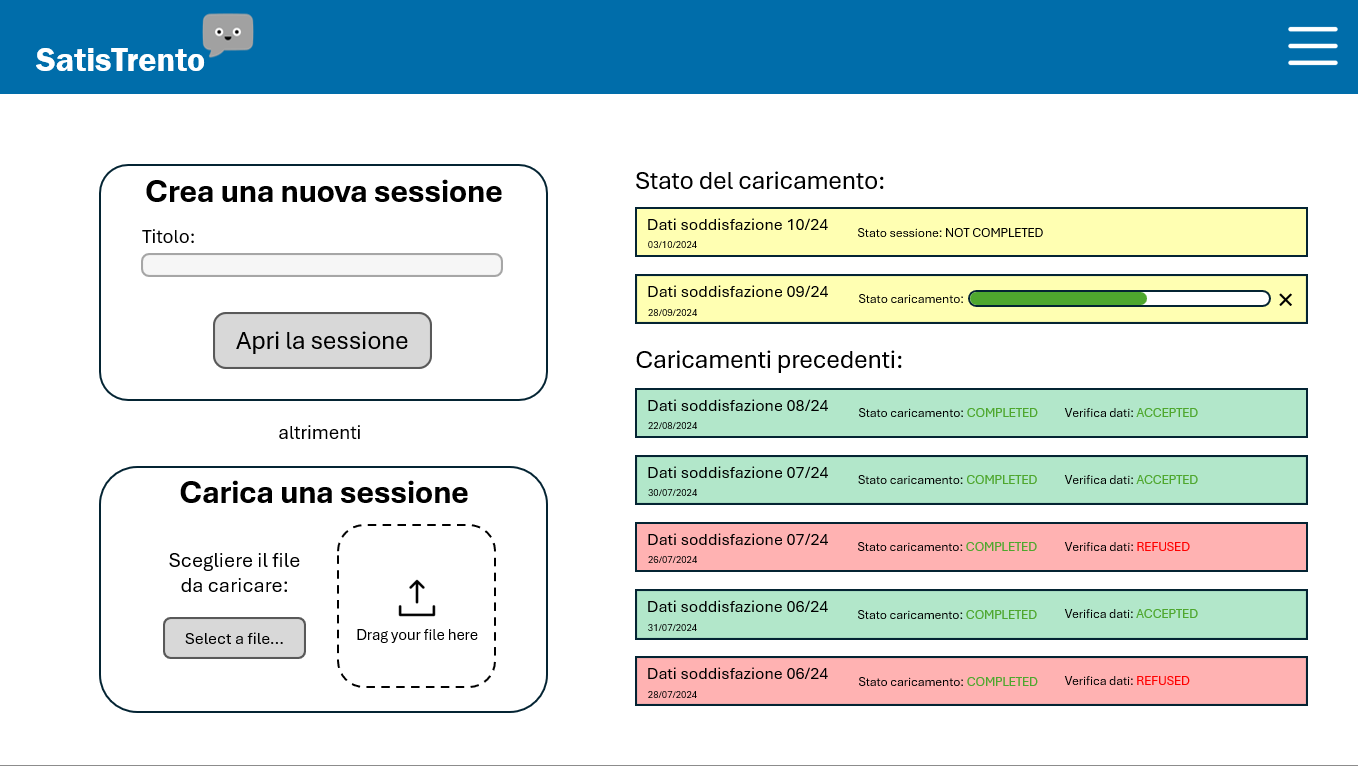
\includegraphics[width=0.6\textwidth]{Interfaccia_grafica/VisSondaggi.png}
        \caption{Caricamento dati e visualizzazione elenco}
    \end{figure} 
    La figura 4.4 mostra il mockup della schermata visibile ai sondaggisti.\newline
    Il presente layout sarà inoltre la base per le visualizzazioni lato amministratore per la valutazione dei sondaggi.
    \begin{itemize}
        \item \textbf{RF8: Visualizzazione sondaggi} \begin{itemize}
            \item La seguente pagina permetterà ai sondaggisti di visualizzare lo stato di caricamento dei propri sondaggi. All'interno della visualizzazione sono presenti le liste contenenti i sondaggi in corso e i sondaggi caricati, con corrispettivo stato di approvazione, e l'interfaccia per aggiungere nuovi sondaggi.
        \end{itemize}
        \item \textbf{RF9: Gestione sondaggi} \begin{itemize}
            \item Nella parte sinistra del mockup si può notare come, al fine di caricare un sondaggio se ne possa creare uno inserendogli un nome o come se ne possa caricare uno tramite selezione oppure tramire pull and drag.
            \item Possiamo inoltre notare che in assenza di ulteriori pulsanti al fine di selezionare un sonaggio è sufficente cliccare su di un sondaggio in corso per poter passare alla sua interfaccia.
        \end{itemize}
        \item \textbf{RNF6: Capacità di caricamento} \begin{itemize}
            \item Questa sarà la principale pagina di caricamento dati sull'applicazione una volta che sull'applicazione saranno caricati i dati di base. In quanto i dati dei sondaggi potrebbero essere pesanti e numerosi, l'interfaccia dovrà essere in grado di gestire il caricamento di grandi quantità di dati in breve tempo.
        \end{itemize}
        \item \textbf{RNF10: Facilità d'uso} \begin{itemize}
            \item Si nota come l'interfaccia è intuitiva e permette all'utente di capire facilmente come caricare i dati e come vedere l'elenco delle informazioni già caricate.
        \end{itemize}
    \end{itemize}

\section{Creazione nuovo sondaggio}

    \begin{figure}[H]
        \center
        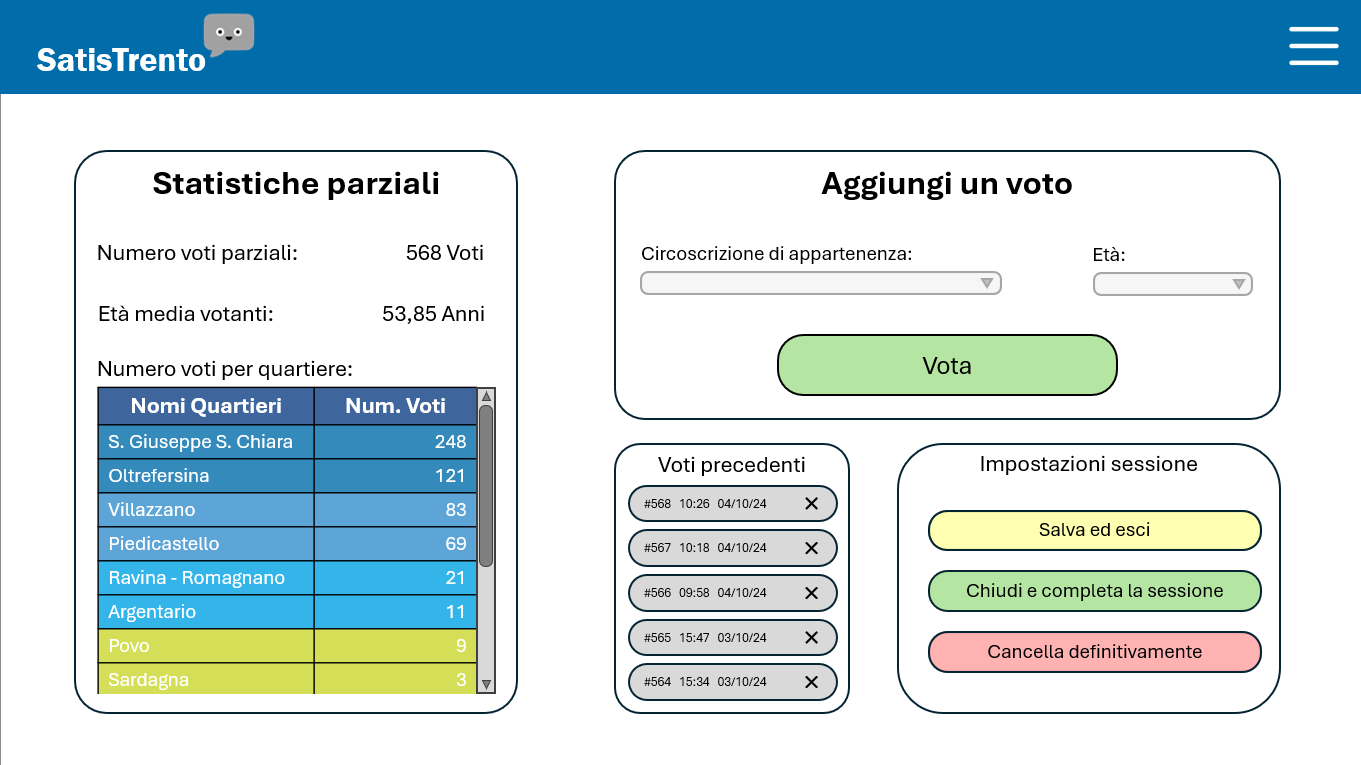
\includegraphics[width=0.6\textwidth]{Interfaccia_grafica/VisVoti.png}
        \caption{Schermata della sessione di sondaggio}
    \end{figure}

    La figura 4.5 mostra il mockup della schermata visibile ai sondaggisti durante una sessione di sondaggio. L'interfaccia mostra informazioni sul sondaggio attuale.

    \begin{itemize}
        \item \textbf{RF9: Gestione sondaggi} \begin{itemize}
            \item Nell'angolo in basso a destra del mockup possiamo notare, colorati di diversi colori, i pulsanti necessari per gestire la sessione di un sondaggio, in giallo è presente il pulsante per salvare la sessione in modo da poterla continuare in futuro, in verde vi è il pulsante per caricare a sistema la sessione ed infine in rosso vi è il pulsante per cancellare la sessione e tutti i voti a se annessi.
        \end{itemize}
        \item \textbf{RF10: Visualizzazione voti} \begin{itemize}
            \item Possiamo notare come nella parte sinistra dell'interfaccia presentata sia presente la sezione denominata "statistiche parziali". Tale sezione permette di visualizzare in primo piano le statistiche principali come il numero di voti raccolti all'interno del sondaggio, oppure l'età media dei votanti e subito sotto permette di visualizzare una lista relativa alla provenienza delle persone che hanno votato all'interno del sondaggio.
            \item Nella parte destra dell'interfaccia vi sono le sottointerfacce per la gestione dei voti e per la gestione dei sondaggi.
        \end{itemize}
        \item \textbf{RF11: Gestione voti} \begin{itemize}
            \item All'interno del mockup, nella parte destra di schermo è possibile visualizzare le due interfacce per la gestione dei voti. In alto vi è l'interfaccia per aggiungere i voti, con rispettivi campi e pulsanti mentre in basso vi è la lista degli ultimi voti caricati.
        \end{itemize}
    \end{itemize}
    